\begin{lstlisting}
Section 8.3:  4, 9, 15, 21 (ed7:4, 7,12, 18)
Section 9.2: 1, 5, 8 (ed7: 2, 5 , 7)  
Section 9.5:  7, 10  (ed7: 6, 9)
\end{lstlisting}
\begin{exercise}
\begin{figure}[H]
\centering
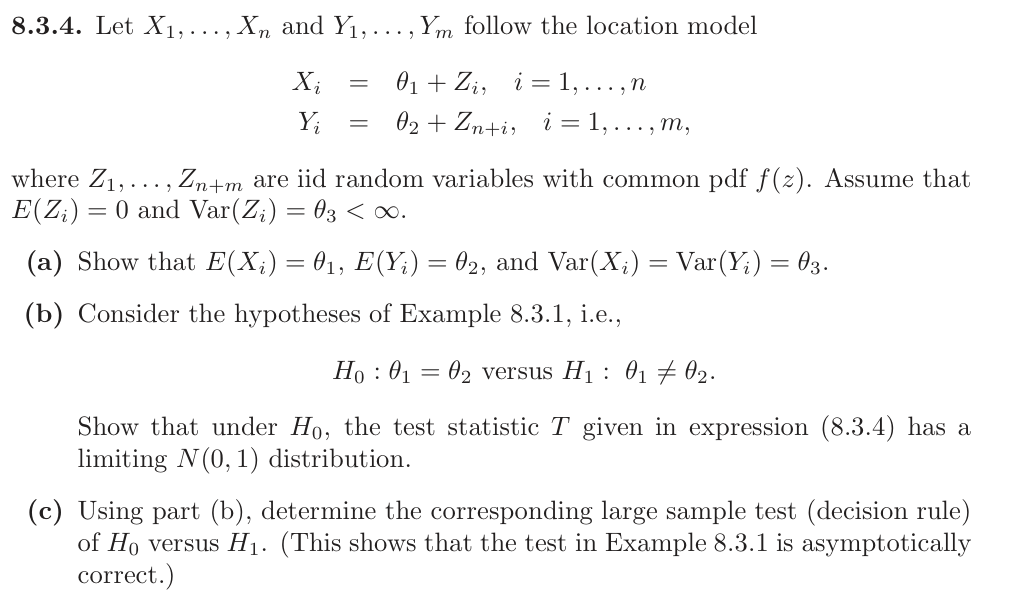
\includegraphics[width=\textwidth]{hw15-2025061519.png}
% \caption{}
\label{}
\end{figure}
\end{exercise}
(a) 显然

(b)
\[
T=\sqrt{\frac{n m}{n+m}}(\bar{X}-\bar{Y})\left\{(n+m-2)^{-1}\left[\sum_1^n\left(X_i-\bar{X}\right)^2+\sum_1^m\left(Y_i-\bar{Y}\right)^2\right]\right\}^{-1 / 2}
\]
设 $\overline{Z}=\frac{1}{n}\sum_{i=1}^{n}Z_i$,$\overline{W}=\frac{1}{m}\sum_{i=1}^{m}Z_{n+i}$,于是
\[
T=\sqrt{ \frac{nm}{n+m} }(\overline{Z}-\overline{W})\left\{  (n+m-2)^{-1}\left[ \sum_{i=1}^{n} (Z_i-\overline{Z})^{2}+\sum_{i=1}^{m} (Z_{n+i}-\overline{W})^{2} \right]  \right\}^{-1/2 }
\]
$\mathrm{Var}(\overline{Z})=\frac{1}{n}\theta_3$, $\mathrm{Var}(\overline{W})=\frac{1}{m}\theta_3$. Then $\mathrm{Var}(\overline{Z}-\overline{W})=\left( \frac{1}{n}+\frac{1}{m} \right)\theta_3$. By CLT,
\[
\frac{\overline{Z}-\overline{W}}{\sqrt{ \left( \frac{1}{n}+\frac{1}{m}  \right)\theta_3}}\overset{ \mathcal{D} }{ \to }N(0,1)
\]
Thus $\sqrt{ \frac{nm}{n+m} }(\overline{Z}-\overline{W})\overset{ \mathcal{D} }{ \to }\sqrt{ \theta_3 }N(0,1)$. By the Law of Large Numbers, as $n\to \infty$, $S_{Z}^{2}=\frac{1}{n-1}\sum_{i=1}^{n}(Z_i-\overline{Z})^{2}\overset{ \mathcal{P} }{ \to }\mathrm{Var}(Z_i)=\theta_3$. And $S_{W}^{2}=\frac{1}{m-1}\sum_{i=1}^{m}(Z_{n+i}-\overline{W})^{2}\overset{ \mathcal{P} }{ \to }\mathrm{Var}(Z_{n+i})=\theta_3$. Thus $S_{p}^{2}=\frac{(n-1)S_{Z}^{2}+(m-1)S_{W}^{2}}{n+m-2}\overset{ \mathcal{P} }{ \to }\theta_3$.

By Slutsky's theorem, $\sqrt{ \frac{nm}{n+m} }\frac{\overline{Z}-\overline{W}}{\sqrt{ \theta_3 }}\cdot\frac{\sqrt{ \theta_3 }}{\sqrt{ S_{p}^{2} }}\overset{ \mathcal{D} }{ \to }N(0,1)$.

(c)
Since, under $H_0$, the test statistic $T$ asymptotically follows a standard normal distribution $N(0,1)$, we can use the quantiles of the standard normal distribution to construct a large sample test.

We reject $H_0$ at level $\alpha$ if $\lvert T \rvert>z_{\alpha/2 }$.

\begin{exercise}
\begin{figure}[H]
\centering
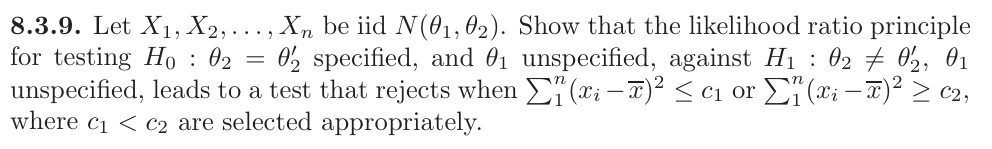
\includegraphics[width=\textwidth]{1-hw15-2025061519.png}
% \caption{}
\label{}
\end{figure}
\end{exercise}
\[
L\left(\theta_1, \theta_2\right)=\prod_{i=1}^n \frac{1}{\sqrt{2 \pi \theta_2}} \exp \left(-\frac{\left(x_i-\theta_1\right)^2}{2 \theta_2}\right)=\left(2 \pi \theta_2\right)^{-n / 2} \exp \left(-\frac{1}{2 \theta_2} \sum_{i=1}^n\left(x_i-\theta_1\right)^2\right)
\]
The likelihood ratio test statistic $\Lambda$ is defined as:
\[
\Lambda=\frac{\sup_{\boldsymbol{\theta}\in\Theta_0}L(\boldsymbol{\theta})}{\sup_{\boldsymbol{\theta}\in\Theta}L(\boldsymbol{\theta})}
\]
Let
\[
\frac{\partial \ln L}{\partial \theta_1}=-\frac{1}{2 \theta_2} \sum_{i=1}^n 2\left(x_i-\theta_1\right)(-1)=\frac{1}{\theta_2} \sum_{i=1}^n\left(x_i-\theta_1\right)=0
\]
\[
\frac{\partial \ln L}{\partial \theta_2}=-\frac{n}{2 \theta_2}+\frac{1}{2 \theta_2^2} S^2=0
\]
Then $\widehat{\theta_1}=\overline{x}$, $\widehat{\theta_2}=\frac{1}{n}S^{2}=\frac{1}{n}\sum_{i=1}^{n}(x_i-\overline{x})^{2}$.
\[
L\left(\hat{\theta}_1, \hat{\theta}_2\right)=(2 \pi)^{-n / 2}\left(\frac{S^2}{n}\right)^{-n / 2} \exp \left(-\frac{n S^2}{2 S^2}\right)=(2 \pi)^{-n / 2}\left(\frac{S^2}{n}\right)^{-n / 2} \exp \left(-\frac{n}{2}\right)
\]
Under $H_0$, the likelihood function becomes:
\[
L\left(\theta_1, \theta_2^{\prime}\right)=\left(2 \pi \theta_2^{\prime}\right)^{-n / 2} \exp \left(-\frac{1}{2 \theta_2^{\prime}} \sum_{i=1}^n\left(x_i-\theta_1\right)^2\right)
\]
We need to maximize this with respect to $\theta_1$. As before, the MLE for $\theta_1$ is $\hat{\theta}_{1,0}=\bar{x}$. So, the maximized likelihood under $H_0$ is:
\[
L\left(\hat{\theta}_{1,0}, \theta_2^{\prime}\right)=L\left(\bar{x}, \theta_2^{\prime}\right)=\left(2 \pi \theta_2^{\prime}\right)^{-n / 2} \exp \left(-\frac{1}{2 \theta_2^{\prime}} \sum_{i=1}^n\left(x_i-\bar{x}\right)^2\right)
\]
\[
L\left(\hat{\theta}_{1,0}, \theta_2^{\prime}\right)=\left(2 \pi \theta_2^{\prime}\right)^{-n / 2} \exp \left(-\frac{S^2}{2 \theta_2^{\prime}}\right)
\]
Therefore the likelihood ratio statistic $\Lambda$ is
\[
\Lambda=\left(\frac{S^2}{n \theta_2^{\prime}}\right)^{n / 2} \exp \left(\frac{n}{2}-\frac{S^2}{2 \theta_2^{\prime}}\right)
\]
which is a increasing function of $S^{2}$. Then $\Lambda\geq c$ iff $S^{2}\geq c'$ for some $c'$. By Student's theorem, we have $\frac{1}{\theta_2'}S^{2}\sim \chi^{2}(n-1)$. Then the rejection region is
\[
\frac{1}{\theta_2'}S^{2}\leq \chi^{2}_{\alpha/2,n-1}\text{ or }\frac{1}{\theta_2'}S^{2}\geq \chi^{2}_{1-\alpha/2,n-1}
\]
i.e.
\[
S^{2}\leq \theta_2'\chi^{2}_{\alpha/2,n-1}\text{ or }S^{2}\geq \theta_2'\chi^{2}_{1-\alpha/2,n-1}
\]
\begin{exercise}
\begin{figure}[H]
\centering
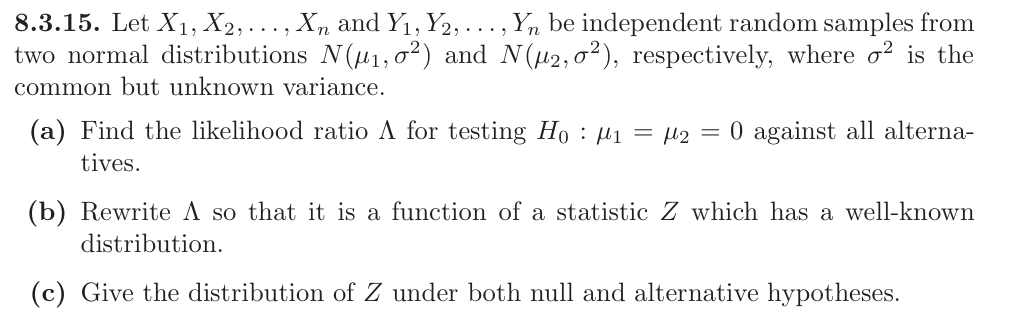
\includegraphics[width=\textwidth]{2-hw15-2025061519.png}
% \caption{}
\label{}
\end{figure}
\end{exercise}
\begin{figure}[H]
\centering
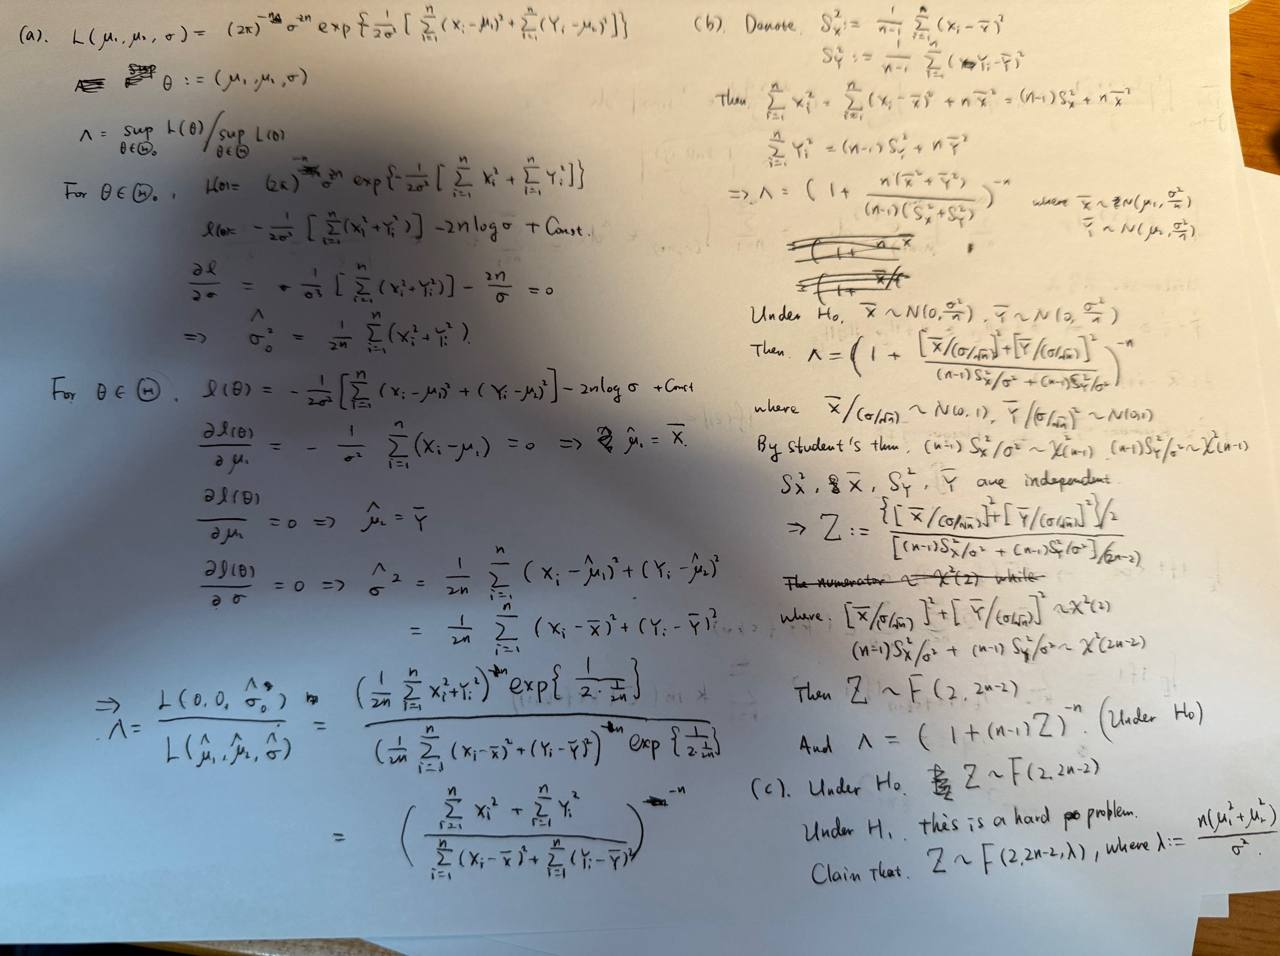
\includegraphics[width=\textwidth]{hw15-2025061523.png}
% \caption{}
\label{}
\end{figure}

Under $H_1$,
\[
Z=\frac{\{ [ \overline{X}/(\sigma/\sqrt{ n })]^{2}+[\overline{Y}/(\sigma/\sqrt{ n })]^{2} \}/2}{[(n-1)S_{X}^{2}/\sigma^{2}+(n-1)S_{Y}^{2}/\sigma^{2}]/(2n-2)}
\]
where $\overline{X}/(\sigma/\sqrt{ n })\sim N(\mu_1/(\sigma/\sqrt{ n }),1)$ and $\overline{Y}/(\sigma/\sqrt{ n })\sim N(\mu_2/(\sigma/\sqrt{ n }),1)$. By the definition of noncentral chi-square distribution,
\[
\left[ \overline{X}/(\sigma/\sqrt{ n }) \right]^{2}+[\overline{Y}/(\sigma/\sqrt{ n })]^{2}\sim \chi^{2}(2,\lambda)
\]
where $\lambda=\frac{\mu_1^{2}+\mu_2^{2}}{(\sigma/\sqrt{ n })^{2}}=\frac{n(\mu_1^{2}+\mu_2^{2})}{\sigma^{2}}$. Thus $Z\sim F(2,2n-2,\lambda)$.

\begin{exercise}
\begin{figure}[H]
\centering
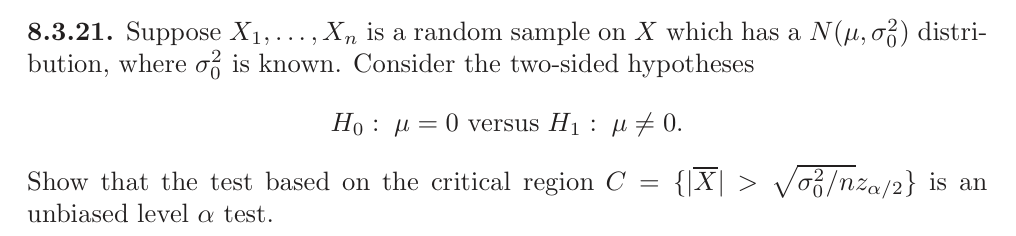
\includegraphics[width=\textwidth]{3-hw15-2025061519.png}
% \caption{}
\label{}
\end{figure}
\end{exercise}
Under $H_0$, $\mathbb{P}_{H_0}(\mathbf{X}\in C)=\mathbb{P}_{H_0}\left( \left\lvert  \frac{\overline{X}}{\sqrt{ \sigma_0^{2}/n }}  \right\rvert>z_{\alpha/2 } \right)=\alpha$.
\[
\overline{X}=\mu+\sqrt{ \sigma_0^{2}/n }\cdot Z\sim N\left( \mu,\frac{\sigma_0^{2}}{n} \right)
\]
where $Z\sim N(0,1)$. Then
\[
\begin{aligned}
C & =\{ \lvert \overline{X} \rvert >\sqrt{ \sigma_0^{2}/n }z_{\alpha/2 } \} \\
 & =\{ \lvert \mu+\sqrt{ \sigma_0^{2}/n }Z \rvert >\sqrt{ \sigma_0^{2}/n }z_{\alpha/2 } \} \\
 & \overset{ c\coloneqq \mu/\sqrt{ \sigma_0^{2}/n } }{ = }\{ Z>z_{\alpha/2 }-c \}\cup \{ Z<-z_{\alpha/2 }-c \} 
\end{aligned}
\]
For any $\mu\neq0$, we have $c\neq0$. Then
\[
\begin{aligned}
\mathbb{P}_{\mu}(\mathbf{X}\in C) & =\mathbb{P}(Z>z_{\alpha/2 }-c)+\mathbb{P}(Z<-z_{\alpha/2 }-c) \\
 & =\mathbb{P}(Z>z_{\alpha/2 })+\mathbb{P}(z_{\alpha/2 }-c<Z\leq z_{\alpha/2  })+\mathbb{P}(Z<-z_{\alpha/2 })-\mathbb{P}(-z_{\alpha/2 }-c\leq Z<-z_{\alpha/2 }) \\
 & =\alpha+\mathbb{P}(z_{\alpha/2 }-c<Z\leq z_{\alpha/2  })-\mathbb{P}(-z_{\alpha/2 }-c\leq Z<-z_{\alpha/2 }) \\
 & =\alpha+\mathbb{P}(z_{\alpha/2 }-c<Z\leq z_{\alpha/2  })-\mathbb{P}(z_{\alpha/ 2 }<Z\leq z_{\alpha/2  }+c) \\
 & \geq \alpha
\end{aligned}
\]
Thus the test beased on the critical region $C$ is an unbiased level $\alpha$ test.

\begin{exercise}
\begin{figure}[H]
\centering
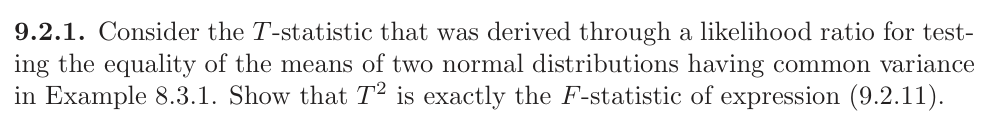
\includegraphics[width=\textwidth]{4-hw15-2025061519.png}
% \caption{}
\label{}
\end{figure}
\end{exercise}
\[
T=\sqrt{\frac{n m}{n+m}}(\bar{X}-\bar{Y})\left\{(n+m-2)^{-1}\left[\sum_1^n\left(X_i-\bar{X}\right)^2+\sum_1^m\left(Y_i-\bar{Y}\right)^2\right]\right\}^{-1 / 2}
\]
\[
T^2=\frac{n m}{n+m}(\bar{X}-\bar{Y})^2 \frac{(n+m-2)}{\sum_1^n\left(X_i-\bar{X}\right)^2+\sum_1^m\left(Y_i-\bar{Y}\right)^2}
\]
In (9.2.11),
\[
F=\frac{Q_4/(b-1)}{Q_3/(n-b)}
\]
where
\[
Q_3=\sum_{j=1}^{b} \sum_{i=1}^{n_j} (x_{ij}-\overline{x}_{\cdot j})^{2}
\]
\[
Q_4=\sum_{j=1}^{b} n_j(\overline{x}_{\cdot j}-\overline{x}_{\cdot \cdot })^{2}
\]
Let $j=2$, and $x_{i 1}=X_i$ for $i=1,\dots,n$, $x_{i 2}=Y_i$ for $i=1,\dots,m$. Then
\[
\overline{x}_{\cdot1}=\overline{X},\qquad \overline{x}_{\cdot 2}=\overline{Y}
\]
\[
\overline{x}_{\cdot \cdot }=\frac{n\overline{x}_{\cdot 1}+m\overline{x}_{\cdot 2}}{n+m}=\frac{n\overline{X}+m\overline{Y}}{n+m}
\]
Then
\[
Q_4=n\left( \overline{X}-\frac{n\overline{X}+m\overline{Y}}{n+m} \right)^{2}+m\left( \overline{Y}-\frac{n\overline{X}+m\overline{Y}}{n+m} \right)^{2}=\frac{mn}{m+n}(\overline{X}-\overline{Y})^{2}
\]
\[
Q_3=\sum_{i=1}^{n} (X_i-\overline{X})^{2}+\sum_{i=1}^{m} (Y_i-\overline{Y})^{2}
\]
\[
b-1=1,\qquad n+m-b=m+n-2
\]
Thus
\[
T^{2}=F
\]
for $j=2$, and $x_{i 1}=X_i$ for $i=1,\dots,n$, $x_{i 2}=Y_i$ for $i=1,\dots,m$.

\begin{exercise}
\begin{figure}[H]
\centering
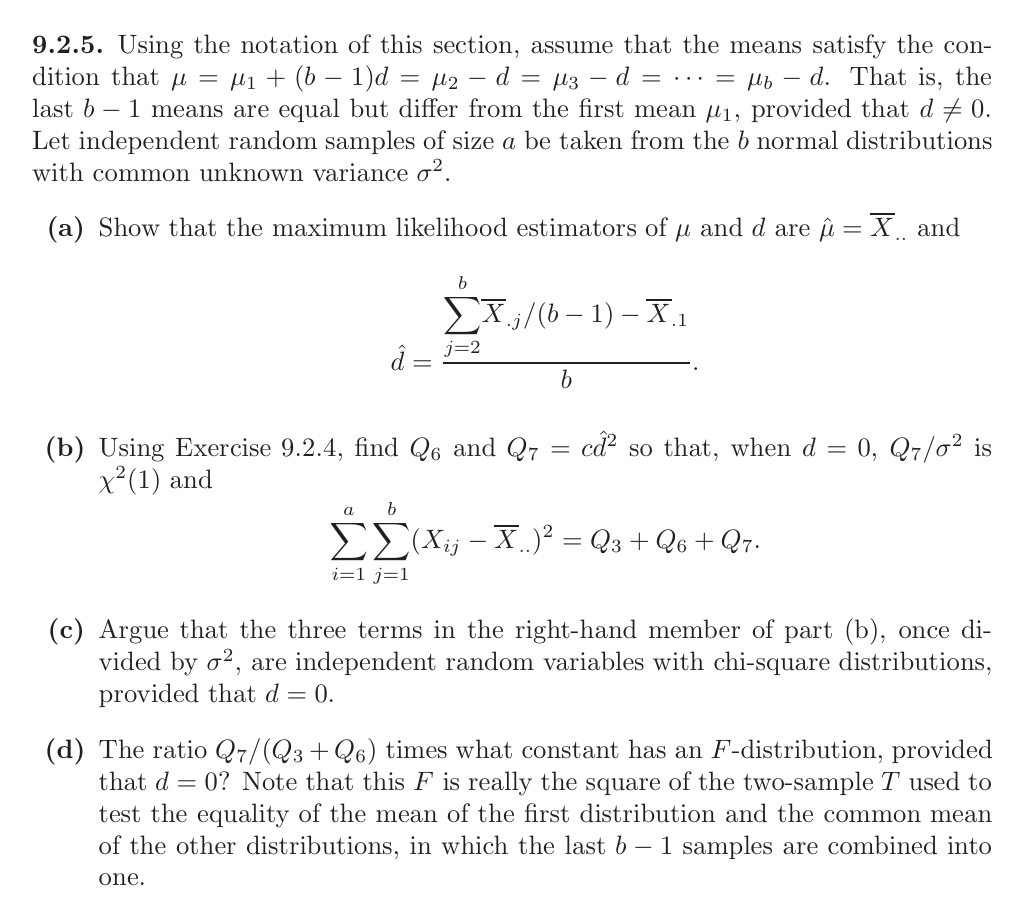
\includegraphics[width=\textwidth]{5-hw15-2025061519.png}
% \caption{}
\label{}
\end{figure}
\end{exercise}
(a)
\begin{figure}[H]
\centering
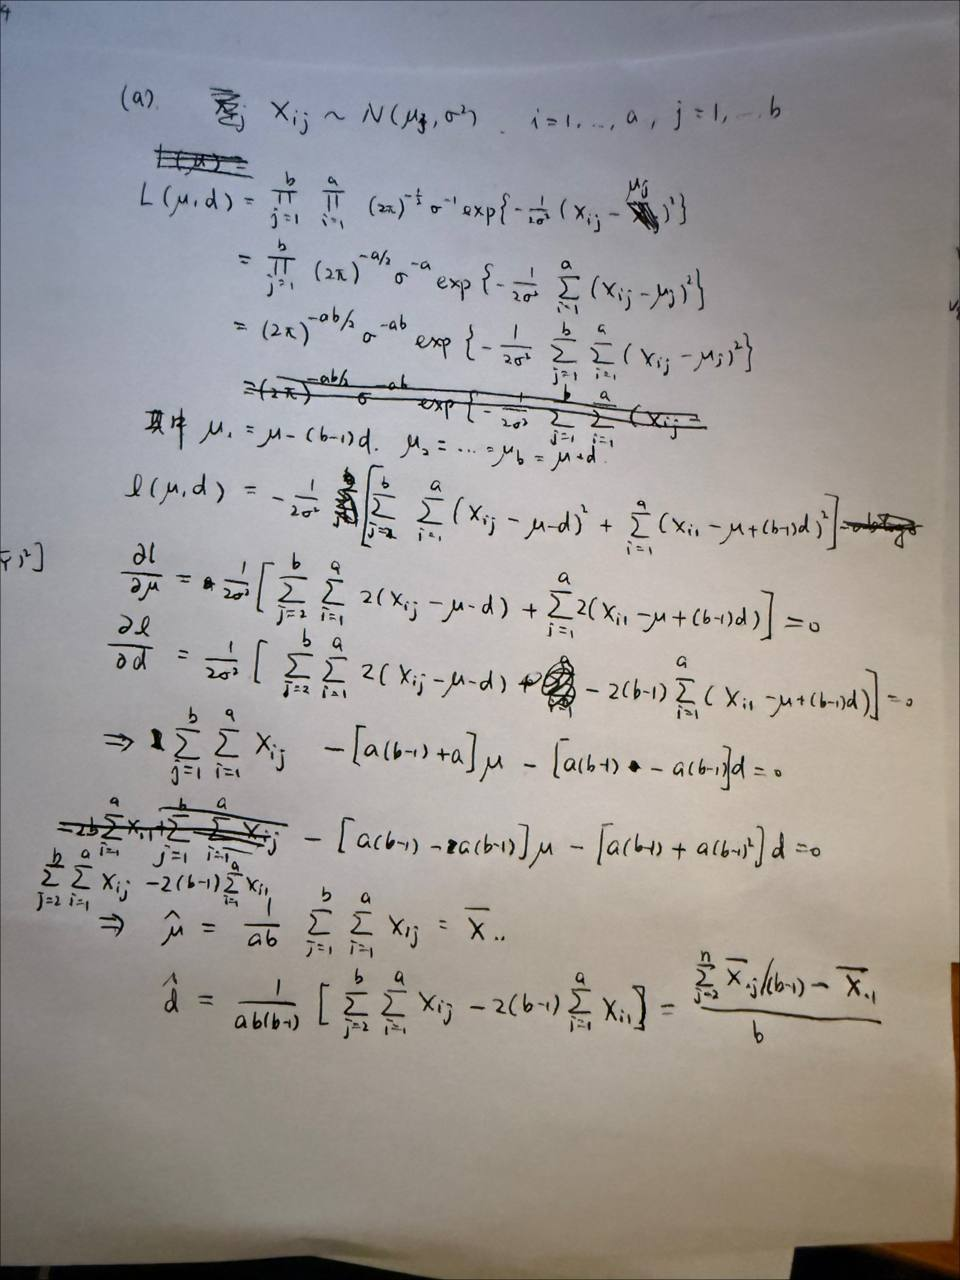
\includegraphics[width=\textwidth]{hw15-2025061700.png}
% \caption{}
\label{}
\end{figure}
(b)(c)
\begin{figure}[H]
\centering
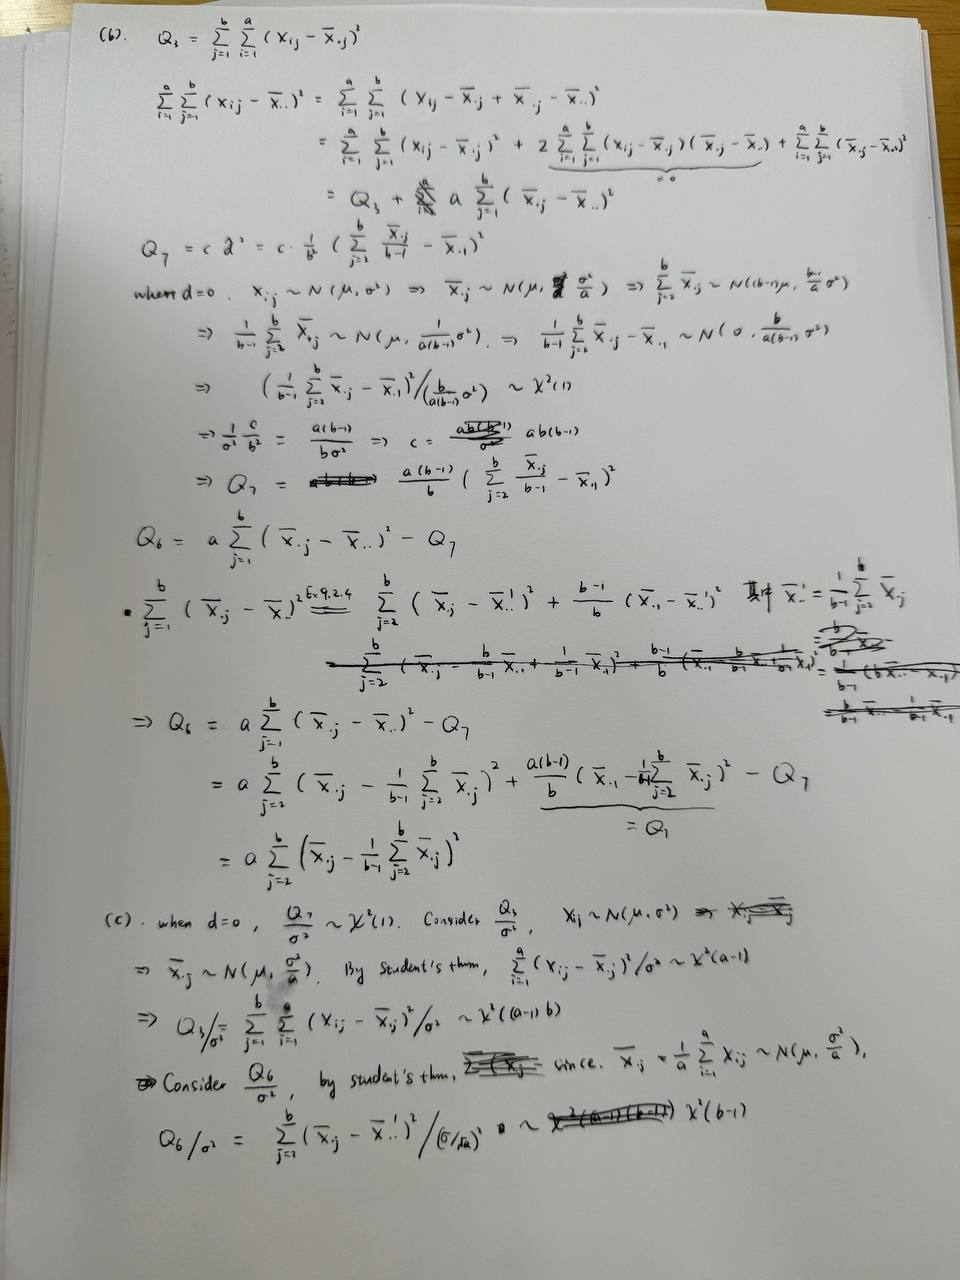
\includegraphics[width=\textwidth]{1-hw15-2025061711.png}
% \caption{}
\label{}
\end{figure}
(d)
\begin{figure}[H]
\centering
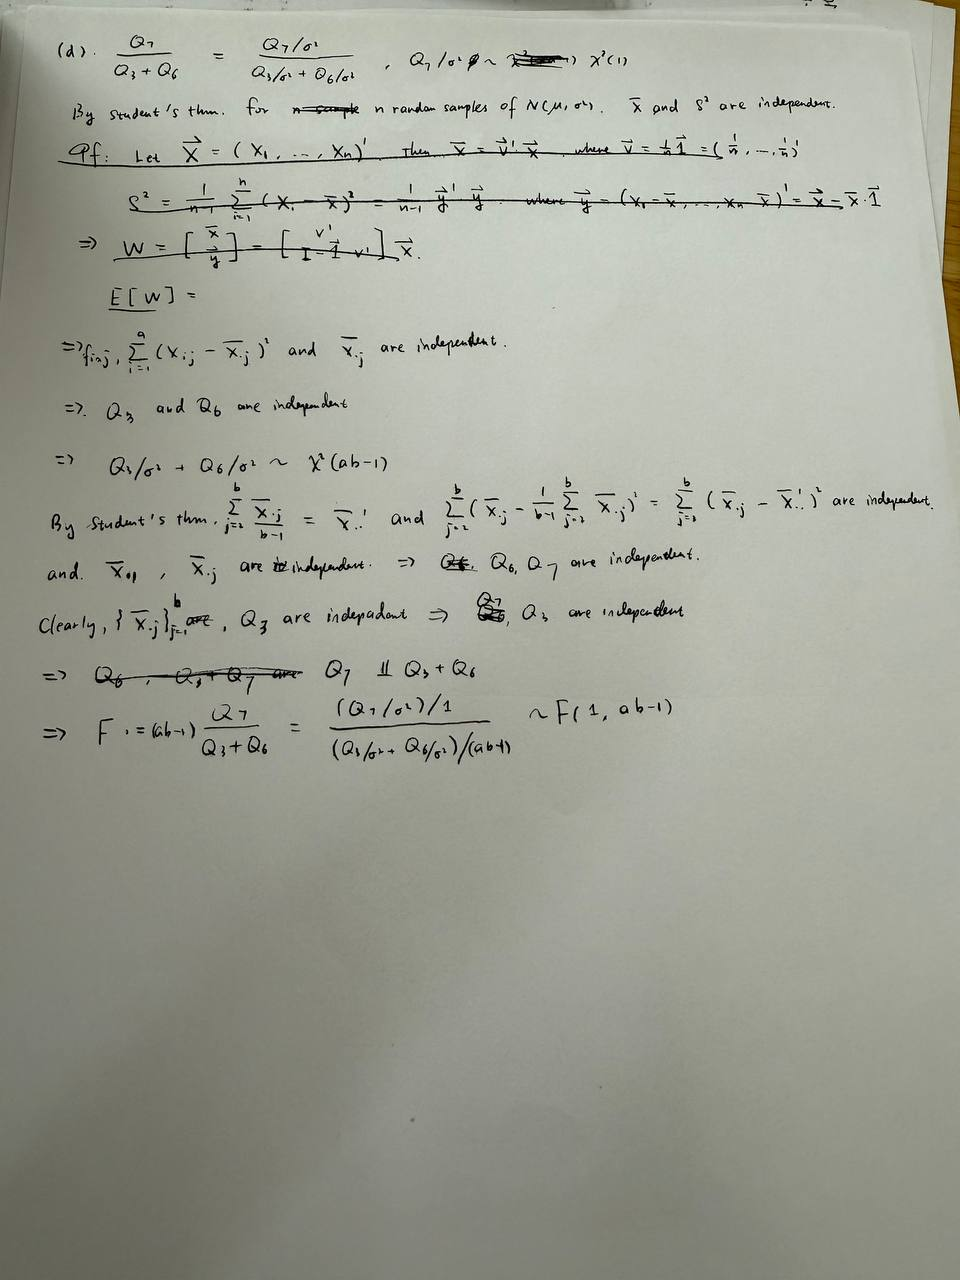
\includegraphics[width=\textwidth]{2-hw15-2025061711.png}
% \caption{}
\label{}
\end{figure}

\begin{exercise}
\begin{figure}[H]
\centering
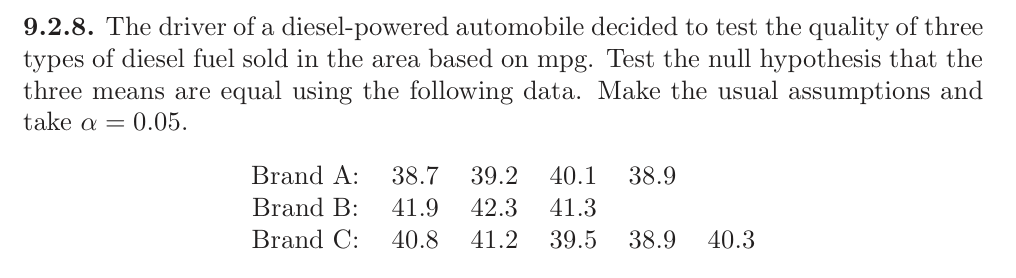
\includegraphics[width=\textwidth]{6-hw15-2025061519.png}
% \caption{}
\label{}
\end{figure}
\end{exercise}
To test the null hypothesis that the three means are equal, we can use a one-way Analysis of Variance (ANOVA).

Given data:
Brand A: 38.7, 39.2, 40.1, 38.9

Brand B: 41.9, 42.3, 41.3

Brand C: 40.8, 41.2, 39.5, 38.9, 40.3

\begin{enumerate}
	\item State the null and alternative hypotheses.
\[
H_0: \mu_A = \mu_B = \mu_C \text{ (The means of mpg for the three brands of diesel fuel are equal)}
\]\[
H_1: \text{At least one mean is different}
\]	\item Calculate the sample means for each brand.
\[
\widehat{x}_A = (38.7 + 39.2 + 40.1 + 38.9) / 4 = 156.9 / 4 = 39.225
\]\[
\widehat{x}_B = (41.9 + 42.3 + 41.3) / 3 = 125.5 / 3 = 41.833
\]\[
\widehat{x}_C = (40.8 + 41.2 + 39.5 + 38.9 + 40.3) / 5 = 200.7 / 5 = 40.14
\]	\item Calculate the overall mean (grand mean).
Total number of observations $N = 4 + 3 + 5 = 12$
Sum of all observations $= 38.7 + 39.2 + 40.1 + 38.9 + 41.9 + 42.3 + 41.3 + 40.8 + 41.2 + 39.5 + 38.9 + 40.3 = 483.1$
\[
\overline{\overline{x}} = 483.1 / 12 = 40.258
\]	\item Calculate the Sum of Squares Between (SSB) treatments.
$n_A = 4$, $n_B = 3$, $n_C = 5$
\[
SSB = n_A(\widehat{x}_A - \overline{\overline{x}})^2 + n_B(\widehat{x}_B - \overline{\overline{x}})^2 + n_C(\widehat{x}_C - \overline{\overline{x}})^2
\]\[
SSB = 4(39.225 - 40.258)^2 + 3(41.833 - 40.258)^2 + 5(40.14 - 40.258)^2
\]\[
SSB = 4(-1.033)^2 + 3(1.575)^2 + 5(-0.118)^2
\]\[
SSB = 4(1.067089) + 3(2.480625) + 5(0.013924)
\]\[
SSB = 4.268356 + 7.441875 + 0.06962 = 11.779851
\]	\item Calculate the Sum of Squares Within (SSW) treatments (Error Sum of Squares).
For Brand A: $(38.7-39.225)^2 + (39.2-39.225)^2 + (40.1-39.225)^2 + (38.9-39.225)^2$
\[
= (-0.525)^2 + (-0.025)^2 + (0.875)^2 + (-0.325)^2
\]\[
= 0.275625 + 0.000625 + 0.765625 + 0.105625 = 1.1475
\]For Brand B: $(41.9-41.833)^2 + (42.3-41.833)^2 + (41.3-41.833)^2$
\[
= (0.067)^2 + (0.467)^2 + (-0.533)^2
\]\[
= 0.004489 + 0.218089 + 0.284089 = 0.506667
\]For Brand C: $(40.8-40.14)^2 + (41.2-40.14)^2 + (39.5-40.14)^2 + (38.9-40.14)^2 + (40.3-40.14)^2$
\[
= (0.66)^2 + (1.06)^2 + (-0.64)^2 + (-1.24)^2 + (0.16)^2
\]\[
= 0.4356 + 1.1236 + 0.4096 + 1.5376 + 0.0256 = 3.532
\]\[
SSW = 1.1475 + 0.506667 + 3.532 = 5.186167
\]	\item Calculate the Degrees of Freedom.
Degrees of freedom between groups ($df_B$) $= k - 1 = 3 - 1 = 2$ (where $k$ is the number of groups)
Degrees of freedom within groups ($df_W$) $= N - k = 12 - 3 = 9$
Total degrees of freedom ($df_T$) $= N - 1 = 12 - 1 = 11$
	\item Calculate the Mean Squares.
Mean Square Between ($MSB$)
\[
= SSB / df_B = 11.779851 / 2 = 5.8899255
\]Mean Square Within ($MSW$)
\[
= SSW / df_W = 5.186167 / 9 = 0.57624077
\]	\item Calculate the F-statistic.
\[
F = MSB / MSW = 5.8899255 / 0.57624077 = 10.2212
\]	\item Determine the critical F-value.
Using $\alpha=0.05$, $df_1 = 2$, and $df_2 = 9$.
From the F-distribution table, the critical F-value is approximately $F_{0.05, 2, 9} = 4.26$.
	\item Make a decision.
Since the calculated F-statistic (10.2212) is greater than the critical F-value (4.26), we reject the null hypothesis.
\end{enumerate}

Conclusion:
At a 0.05 level of significance, there is sufficient evidence to conclude that at least one of the mean mpg for the three types of diesel fuel is different.

\begin{exercise}
\begin{figure}[H]
\centering
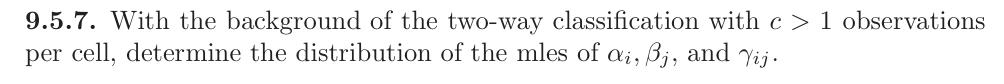
\includegraphics[width=\textwidth]{7-hw15-2025061519.png}
% \caption{}
\label{}
\end{figure}
\end{exercise}
Let's revisit the log-likelihood function:
\[
\ln L = -\frac{abc}{2} \ln(2\pi) - \frac{abc}{2} \ln(\sigma^2) - \frac{1}{2\sigma^2} \sum_{i=1}^{a} \sum_{j=1}^{b} \sum_{k=1}^{c} (X_{ijk} - (\mu + \alpha_i + \beta_j + \gamma_{ij}))^2
\]
To find the MLEs, we need to maximize this function with respect to $\mu, \alpha_i, \beta_j, \gamma_{ij}$, and $\sigma^2$. This involves taking partial derivatives with respect to each parameter and setting them to zero. We'll also impose the standard identifiability constraints to ensure a unique solution:

\begin{enumerate}
	\item $\sum_{i=1}^{a} \alpha_i = 0$
	\item $\sum_{j=1}^{b} \beta_j = 0$
	\item $\sum_{i=1}^{a} \gamma_{ij} = 0$ for all $j$
	\item $\sum_{j=1}^{b} \gamma_{ij} = 0$ for all $i$
\end{enumerate}

Let $P_{ijk} = \mu + \alpha_i + \beta_j + \gamma_{ij}$. The terms involving the parameters only appear in the sum of squares part. Minimizing the sum of squares is equivalent to maximizing the log-likelihood for these parameters.
\[
S = \sum_{i=1}^{a} \sum_{j=1}^{b} \sum_{k=1}^{c} (X_{ijk} - P_{ijk})^2
\]
\textbf{1. Derivative with respect to $\mu$:}
\[
\frac{\partial S}{\partial \mu} = \sum_{i=1}^{a} \sum_{j=1}^{b} \sum_{k=1}^{c} 2(X_{ijk} - (\mu + \alpha_i + \beta_j + \gamma_{ij}))(-1) = 0
\]
\[
\sum_{i=1}^{a} \sum_{j=1}^{b} \sum_{k=1}^{c} X_{ijk} = \sum_{i=1}^{a} \sum_{j=1}^{b} \sum_{k=1}^{c} (\mu + \alpha_i + \beta_j + \gamma_{ij})
\]
\[
abc \overline{X}_{...} = abc\mu + bc\sum_i \alpha_i + ac\sum_j \beta_j + c\sum_i\sum_j \gamma_{ij}
\]
Applying the constraints ($\sum_i \alpha_i = 0$, $\sum_j \beta_j = 0$, and $\sum_i \sum_j \gamma_{ij} = \sum_j (\sum_i \gamma_{ij}) = \sum_j 0 = 0$):
\[
abc \overline{X}_{...} = abc\widehat{\mu} + 0 + 0 + 0
\]
\[
\widehat{\mu} = \overline{X}_{...}
\]
\textbf{2. Derivative with respect to $\alpha_i$ (for a specific $i_0$):}
\[
\frac{\partial S}{\partial \alpha_{i_0}} = \sum_{j=1}^{b} \sum_{k=1}^{c} 2(X_{i_0jk} - (\mu + \alpha_{i_0} + \beta_j + \gamma_{i_0j}))(-1) = 0
\]
\[
\sum_{j=1}^{b} \sum_{k=1}^{c} X_{i_0jk} = \sum_{j=1}^{b} \sum_{k=1}^{c} (\mu + \alpha_{i_0} + \beta_j + \gamma_{i_0j})
\]
\[
bc \overline{X}_{i_0..} = bc\widehat{\mu} + bc\widehat{\alpha}_{i_0} + c\sum_j \widehat{\beta}_j + c\sum_j \widehat{\gamma}_{i_0j}
\]
Applying the constraints ($\sum_j \widehat{\beta}_j = 0$ and $\sum_j \widehat{\gamma}_{i_0j} = 0$ for a given $i_0$):
\[
bc \overline{X}_{i_0..} = bc\widehat{\mu} + bc\widehat{\alpha}_{i_0} + 0 + 0
\]
Substituting $\widehat{\mu} = \overline{X}_{...}$:
\[
bc \overline{X}_{i_0..} = bc\overline{X}_{...} + bc\widehat{\alpha}_{i_0}
\]
\[
\widehat{\alpha}_{i_0} = \overline{X}_{i_0..} - \overline{X}_{...}
\]
This applies for any $i_0$, so $\widehat{\alpha}_i = \overline{X}_{i..} - \overline{X}_{...}$.

\textbf{3. Derivative with respect to $\beta_j$ (for a specific $j_0$):}

By symmetry with $\alpha_i$:
\[
\frac{\partial S}{\partial \beta_{j_0}} = \sum_{i=1}^{a} \sum_{k=1}^{c} 2(X_{ij_0k} - (\mu + \alpha_i + \beta_{j_0} + \gamma_{ij_0}))(-1) = 0
\]
\[
\sum_{i=1}^{a} \sum_{k=1}^{c} X_{ij_0k} = \sum_{i=1}^{a} \sum_{k=1}^{c} (\mu + \alpha_i + \beta_{j_0} + \gamma_{ij_0})
\]
\[
ac \overline{X}_{.j_0.} = ac\widehat{\mu} + c\sum_i \widehat{\alpha}_i + ac\widehat{\beta}_{j_0} + c\sum_i \widehat{\gamma}_{ij_0}
\]
Applying the constraints ($\sum_i \widehat{\alpha}_i = 0$ and $\sum_i \widehat{\gamma}_{ij_0} = 0$ for a given $j_0$):
\[
ac \overline{X}_{.j_0.} = ac\widehat{\mu} + 0 + ac\widehat{\beta}_{j_0} + 0
\]
Substituting $\widehat{\mu} = \overline{X}_{...}$:
\[
ac \overline{X}_{.j_0.} = ac\overline{X}_{...} + ac\widehat{\beta}_{j_0}
\]
\[
\widehat{\beta}_{j_0} = \overline{X}_{.j_0.} - \overline{X}_{...}
\]
This applies for any $j_0$, so $\widehat{\beta}_j = \overline{X}_{.j.} - \overline{X}_{...}$.

\textbf{4. Derivative with respect to $\gamma_{ij}$ (for a specific $i_0, j_0$):}
\[
\frac{\partial S}{\partial \gamma_{i_0j_0}} = \sum_{k=1}^{c} 2(X_{i_0j_0k} - (\mu + \alpha_{i_0} + \beta_{j_0} + \gamma_{i_0j_0}))(-1) = 0
\]
\[
\sum_{k=1}^{c} X_{i_0j_0k} = \sum_{k=1}^{c} (\mu + \alpha_{i_0} + \beta_{j_0} + \gamma_{i_0j_0})
\]
\[
c \overline{X}_{i_0j_0.} = c\widehat{\mu} + c\widehat{\alpha}_{i_0} + c\widehat{\beta}_{j_0} + c\widehat{\gamma}_{i_0j_0}
\]
Substituting the MLEs for $\widehat{\mu}, \widehat{\alpha}_{i_0}, \widehat{\beta}_{j_0}$:
\[
c \overline{X}_{i_0j_0.} = c(\overline{X}_{...}) + c(\overline{X}_{i_0..} - \overline{X}_{...}) + c(\overline{X}_{.j_0.} - \overline{X}_{...}) + c\widehat{\gamma}_{i_0j_0}
\]
Divide by $c$:
\[
\overline{X}_{i_0j_0.} = \overline{X}_{...} + \overline{X}_{i_0..} - \overline{X}_{...} + \overline{X}_{.j_0.} - \overline{X}_{...} + \widehat{\gamma}_{i_0j_0}
\]
\[
\overline{X}_{i_0j_0.} = \overline{X}_{i_0..} + \overline{X}_{.j_0.} - \overline{X}_{...} + \widehat{\gamma}_{i_0j_0}
\]
\[
\widehat{\gamma}_{i_0j_0} = \overline{X}_{i_0j_0.} - \overline{X}_{i_0..} - \overline{X}_{.j_0.} + \overline{X}_{...}
\]
This applies for any $i_0, j_0$, so $\widehat{\gamma}_{ij} = \overline{X}_{ij.} - \overline{X}_{i..} - \overline{X}_{.j.} + \overline{X}_{...}$.

\textbf{5. Derivative with respect to $\sigma^2$:}
\[
\frac{\partial \ln L}{\partial \sigma^2} = -\frac{abc}{2\sigma^2} + \frac{1}{2(\sigma^2)^2} \sum_{i=1}^{a} \sum_{j=1}^{b} \sum_{k=1}^{c} (X_{ijk} - (\mu + \alpha_i + \beta_j + \gamma_{ij}))^2 = 0
\]
Setting to zero and replacing parameters with their MLEs (since the value of $\sigma^2$ that maximizes the likelihood also maximizes it for the other parameters fixed at their MLEs):
\[
\widehat{\sigma}^2 = \frac{1}{abc} \sum_{i=1}^{a} \sum_{j=1}^{b} \sum_{k=1}^{c} (X_{ijk} - (\widehat{\mu} + \widehat{\alpha}_i + \widehat{\beta}_j + \widehat{\gamma}_{ij}))^2
\]
Since $\widehat{\mu} + \widehat{\alpha}_i + \widehat{\beta}_j + \widehat{\gamma}_{ij} = \overline{X}_{ij.}$, we get:
\[
\widehat{\sigma}^2 = \frac{1}{abc} \sum_{i=1}^{a} \sum_{j=1}^{b} \sum_{k=1}^{c} (X_{ijk} - \overline{X}_{ij.})^2
\]
\textbf{Distribution of the MLEs}

Since the $X_{ijk}$ are assumed to be independent and identically distributed $N(\mu + \alpha_i + \beta_j + \gamma_{ij}, \sigma^2)$, and all the MLEs $\widehat{\mu}, \widehat{\alpha}_i, \widehat{\beta}_j, \widehat{\gamma}_{ij}$ are linear combinations of these normal random variables, they will also be normally distributed.

Let $E[\widehat{\theta}]$ and $Var(\widehat{\theta})$ denote the expected value and variance of an estimator $\widehat{\theta}$.

\textbf{1. Distribution of $\widehat{\mu}$:}
\[
\widehat{\mu} = \frac{1}{abc} \sum_{i=1}^{a} \sum_{j=1}^{b} \sum_{k=1}^{c} X_{ijk}
\]
\[
E[\widehat{\mu}] = \frac{1}{abc} \sum_{i=1}^{a} \sum_{j=1}^{b} \sum_{k=1}^{c} E[X_{ijk}] = \frac{1}{abc} \sum_{i=1}^{a} \sum_{j=1}^{b} \sum_{k=1}^{c} (\mu + \alpha_i + \beta_j + \gamma_{ij})
\]
Using the constraints: $\sum \alpha_i = 0, \sum \beta_j = 0, \sum_i \gamma_{ij} = 0, \sum_j \gamma_{ij} = 0$.
\[
E[\widehat{\mu}] = \frac{1}{abc} (abc\mu + bc\sum_i\alpha_i + ac\sum_j\beta_j + c\sum_i\sum_j\gamma_{ij}) = \frac{1}{abc} (abc\mu + 0 + 0 + 0) = \mu
\]
\[
Var(\widehat{\mu}) = Var\left(\frac{1}{abc} \sum X_{ijk}\right) = \frac{1}{(abc)^2} \sum Var(X_{ijk}) = \frac{abc \sigma^2}{(abc)^2} = \frac{\sigma^2}{abc}
\]
So, $\widehat{\mu} \sim N\left(\mu, \frac{\sigma^2}{abc}\right)$.

\textbf{2. Distribution of $\widehat{\alpha}_i$:}
\[
\widehat{\alpha}_i = \overline{X}_{i..} - \overline{X}_{...}
\]
\[
E[\widehat{\alpha}_i] = E[\overline{X}_{i..}] - E[\overline{X}_{...}]
\]
\[
E[\overline{X}_{i..}] = \frac{1}{bc} \sum_{j=1}^{b} \sum_{k=1}^{c} E[X_{ijk}] = \frac{1}{bc} \sum_{j=1}^{b} \sum_{k=1}^{c} (\mu + \alpha_i + \beta_j + \gamma_{ij})
\]
\[
= \frac{1}{bc} (bc\mu + bc\alpha_i + c\sum_j\beta_j + c\sum_j\gamma_{ij})
\]
Using constraints: $\sum_j\beta_j = 0$ and $\sum_j\gamma_{ij} = 0$.
\[
E[\overline{X}_{i..}] = \frac{1}{bc} (bc\mu + bc\alpha_i) = \mu + \alpha_i
\]
So, $E[\widehat{\alpha}_i] = (\mu + \alpha_i) - \mu = \alpha_i$.

For the variance of $\widehat{\alpha}_i$, we use $Var(Y_1 - Y_2) = Var(Y_1) + Var(Y_2) - 2Cov(Y_1, Y_2)$.
\[
Var(\overline{X}_{i..}) = \frac{\sigma^2}{bc}
\]
\[
Var(\overline{X}_{...}) = \frac{\sigma^2}{abc}
\]
\[
Cov(\overline{X}_{i..}, \overline{X}_{...}) = Cov\left(\frac{1}{bc} \sum_{j=1}^{b}\sum_{k=1}^{c} X_{ijk}, \frac{1}{abc} \sum_{p=1}^{a}\sum_{q=1}^{b}\sum_{r=1}^{c} X_{pqr}\right)
\]
The terms common to both sums are those where $p=i$. So there are $bc$ common terms.
\[
Cov(\overline{X}_{i..}, \overline{X}_{...}) = \frac{1}{bc} \frac{1}{abc} \sum_{j=1}^{b}\sum_{k=1}^{c} Var(X_{ijk}) = \frac{1}{abc^2} \sum_{j=1}^{b}\sum_{k=1}^{c} \sigma^2 = \frac{bc\sigma^2}{abc^2} = \frac{\sigma^2}{abc}
\]
\[
Var(\widehat{\alpha}_i) = \frac{\sigma^2}{bc} + \frac{\sigma^2}{abc} - 2\frac{\sigma^2}{abc} = \frac{\sigma^2}{bc} - \frac{\sigma^2}{abc} = \sigma^2 \left(\frac{a-1}{abc}\right)
\]
So, $\widehat{\alpha}_i \sim N\left(\alpha_i, \sigma^2 \frac{a-1}{abc}\right)$.

\textbf{3. Distribution of $\widehat{\beta}_j$:}

By symmetry with $\widehat{\alpha}_i$:
\[
E[\widehat{\beta}_j] = \beta_j
\]
\[
Var(\widehat{\beta}_j) = \sigma^2 \left(\frac{1}{ac} - \frac{1}{abc}\right) = \sigma^2 \left(\frac{b-1}{abc}\right)
\]
So, $\widehat{\beta}_j \sim N\left(\beta_j, \sigma^2 \frac{b-1}{abc}\right)$.

\textbf{4. Distribution of $\widehat{\gamma}_{ij}$:}
\[
\widehat{\gamma}_{ij} = \overline{X}_{ij.} - \overline{X}_{i..} - \overline{X}_{.j.} + \overline{X}_{...}
\]
\[
E[\widehat{\gamma}_{ij}] = E[\overline{X}_{ij.}] - E[\overline{X}_{i..}] - E[\overline{X}_{.j.}] + E[\overline{X}_{...}]
\]
\[
E[\overline{X}_{ij.}] = \mu + \alpha_i + \beta_j + \gamma_{ij}
\]
So, $E[\widehat{\gamma}_{ij}] = (\mu + \alpha_i + \beta_j + \gamma_{ij}) - (\mu + \alpha_i) - (\mu + \beta_j) + \mu = \gamma_{ij}$.

Calculating the variance of $\widehat{\gamma}_{ij}$ is more complex due to the multiple covariance terms. However, since it is a linear combination of normally distributed random variables, it is also normally distributed. Its variance can be shown to be:
\[
Var(\widehat{\gamma}_{ij}) = \sigma^2 \left( \frac{1}{c} - \frac{1}{bc} - \frac{1}{ac} + \frac{1}{abc} \right) = \sigma^2 \frac{(a-1)(b-1)}{abc}
\]
So, $\widehat{\gamma}_{ij} \sim N\left(\gamma_{ij}, \sigma^2 \frac{(a-1)(b-1)}{abc}\right)$.

\textbf{5. Distribution of $\widehat{\sigma}^2$:}
\[
\widehat{\sigma}^2 = \frac{1}{abc} \sum_{i=1}^{a} \sum_{j=1}^{b} \sum_{k=1}^{c} (X_{ijk} - \overline{X}_{ij.})^2 = \frac{SSE}{abc}
\]
We know that $\frac{SSE}{\sigma^2}$ follows a chi-squared distribution with degrees of freedom equal to $ab(c-1)$.
\[
\frac{abc \widehat{\sigma}^2}{\sigma^2} \sim \chi^2_{ab(c-1)}
\]
These derivations show how the MLEs are obtained by solving the system of equations derived from setting the partial derivatives of the log-likelihood function to zero, incorporating the identifiability constraints. The distributions then follow directly from the properties of linear combinations of normal random variables and the properties of the sum of squared errors.

\begin{exercise}
\begin{figure}[H]
\centering
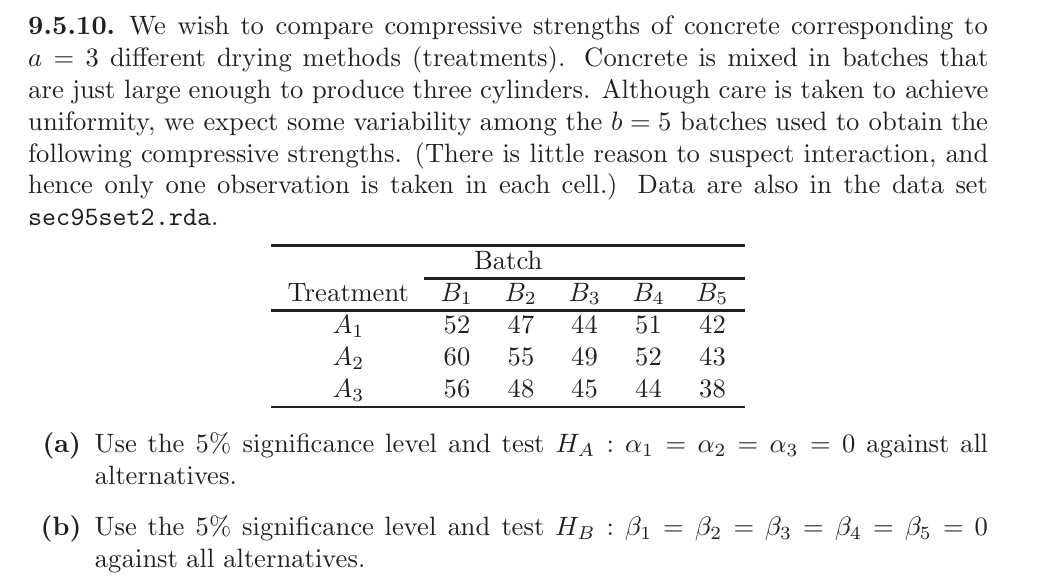
\includegraphics[width=\textwidth]{8-hw15-2025061519.png}
% \caption{}
\label{}
\end{figure}
\end{exercise}
In this problem, we have a two-way ANOVA without replication, as there is only one observation per cell ($c=1$).

The model for this scenario, given that there's little reason to suspect interaction, is typically:
\[
X_{ij} = \mu + \alpha_i + \beta_j + \epsilon_{ij}
\]
where $X_{ij}$ is the observation for the $i$-th treatment and $j$-th batch, $\mu$ is the overall mean, $\alpha_i$ is the effect of the $i$-th treatment, $\beta_j$ is the effect of the $j$-th batch, and $\epsilon_{ij}$ are i.i.d. $N(0, \sigma^2)$ random errors.

We have $a=3$ treatments (drying methods) and $b=5$ batches.

The data are:

\begin{table}[h]
	\centering
	\begin{tabular}{|c|c|c|c|c|c|}
		\hline
		Treatment & $B_1$ & $B_2$ & $B_3$ & $B_4$ & $B_5$ \\
		\hline
		$A_1$ & 52 & 47 & 44 & 51 & 42 \\
		\hline
		$A_2$ & 60 & 55 & 49 & 52 & 43 \\
		\hline
		$A_3$ & 56 & 48 & 45 & 44 & 38 \\
		\hline
	\end{tabular}
\end{table}
First, let's calculate the necessary sums and means.

\textbf{Row Means (Treatment Means):}
\[
\overline{X}_{1.} = (52+47+44+51+42) / 5 = 236 / 5 = 47.2
\]
\[
\overline{X}_{2.} = (60+55+49+52+43) / 5 = 259 / 5 = 51.8
\]
\[
\overline{X}_{3.} = (56+48+45+44+38) / 5 = 231 / 5 = 46.2
\]
\textbf{Column Means (Batch Means):}
\[
\overline{X}_{.1} = (52+60+56) / 3 = 168 / 3 = 56
\]
\[
\overline{X}_{.2} = (47+55+48) / 3 = 150 / 3 = 50
\]
\[
\overline{X}_{.3} = (44+49+45) / 3 = 138 / 3 = 46
\]
\[
\overline{X}_{.4} = (51+52+44) / 3 = 147 / 3 = 49
\]
\[
\overline{X}_{.5} = (42+43+38) / 3 = 123 / 3 = 41
\]
\textbf{Grand Mean:}
Total sum of all observations $= 236 + 259 + 231 = 726$

Number of observations $N = a \times b = 3 \times 5 = 15$
\[
\overline{X}_{..} = 726 / 15 = 48.4
\]
Now, we calculate the sums of squares:

\textbf{Total Sum of Squares ($SST_{Total}$):}
\[
SST_{Total} = \sum_{i=1}^{a} \sum_{j=1}^{b} (X_{ij} - \overline{X}_{..})^2
\]
\[
SST_{Total} = (52-48.4)^2 + (47-48.4)^2 + \dots + (38-48.4)^2
\]
\[
SST_{Total} = (3.6)^2 + (-1.4)^2 + (-4.4)^2 + (2.6)^2 + (-6.4)^2 + (11.6)^2 + (6.6)^2 + (0.6)^2 + (3.6)^2 + (-5.4)^2 + (7.6)^2 + (-0.4)^2 + (-3.4)^2 + (-4.4)^2 + (-10.4)^2
\]
\[
SST_{Total} = 12.96 + 1.96 + 19.36 + 6.76 + 40.96 + 134.56 + 43.56 + 0.36 + 12.96 + 29.16 + 57.76 + 0.16 + 11.56 + 19.36 + 108.16
\]
\[
SST_{Total} = 500.6
\]
\textbf{Sum of Squares for Treatments ($SSTreatments$ or $SSA$):}
\[
SSA = b \sum_{i=1}^{a} (\overline{X}_{i.} - \overline{X}_{..})^2
\]
\[
SSA = 5 \times [(47.2 - 48.4)^2 + (51.8 - 48.4)^2 + (46.2 - 48.4)^2]
\]
\[
SSA = 5 \times [(-1.2)^2 + (3.4)^2 + (-2.2)^2]
\]
\[
SSA = 5 \times [1.44 + 11.56 + 4.84]
\]
\[
SSA = 5 \times 17.84 = 89.2
\]
\textbf{Sum of Squares for Batches ($SSBatches$ or $SSB$):}
\[
SSB = a \sum_{j=1}^{b} (\overline{X}_{.j} - \overline{X}_{..})^2
\]
\[
SSB = 3 \times [(56 - 48.4)^2 + (50 - 48.4)^2 + (46 - 48.4)^2 + (49 - 48.4)^2 + (41 - 48.4)^2]
\]
\[
SSB = 3 \times [57.76 + 2.56 + 5.76 + 0.36 + 54.76]
\]
\[
SSB = 3 \times 121.2 = 363.6
\]
\textbf{Sum of Squares for Error ($SSE$):}
For a two-way ANOVA without replication,
\[
SSE = SST_{Total} - SSA - SSB
\]
\[
SSE = 500.6 - 89.2 - 363.6 = 47.8
\]
\textbf{Degrees of Freedom:}
\[
df_{Total} = N - 1 = 15 - 1 = 14
\]
\[
df_{Treatments} = a - 1 = 3 - 1 = 2
\]
\[
df_{Batches} = b - 1 = 5 - 1 = 4
\]
\[
df_{Error} = (a-1)(b-1) = (3-1)(5-1) = 2 \times 4 = 8
\]
Check: $df_{Treatments} + df_{Batches} + df_{Error} = 2 + 4 + 8 = 14 = df_{Total}$.

\textbf{Mean Squares:}
\[
MS_{Treatments} = SSA / df_{Treatments} = 89.2 / 2 = 44.6
\]
\[
MS_{Batches} = SSB / df_{Batches} = 363.6 / 4 = 90.9
\]
\[
MS_{Error} = SSE / df_{Error} = 47.8 / 8 = 5.975
\]
\textbf{F-statistics:}

\begin{enumerate}
	\item Test $H_A: \alpha_1=\alpha_2=\alpha_3=0$ (No treatment effect)
\[
F_A = MS_{Treatments} / MS_{Error}
\]\[
F_A = 44.6 / 5.975 = 7.464
\]Critical F-value for $F_A$:
\[
F_{0.05, df_{Treatments}, df_{Error}} = F_{0.05, 2, 8}
\]Using an F-table,
\[
F_{0.05, 2, 8} \approx 4.46
\]Decision: Since
\[
F_A = 7.464 > 4.46
\]we reject the null hypothesis $H_A$.
Conclusion for (a): At the $5\%$ significance level, there is sufficient evidence to conclude that there is a significant difference in the compressive strengths of concrete corresponding to the three different drying methods.
	\item Test $H_B: \beta_1=\beta_2=\beta_3=\beta_4=\beta_5=0$ (No batch effect)
\[
F_B = MS_{Batches} / MS_{Error}
\]\[
F_B = 90.9 / 5.975 = 15.213
\]Critical F-value for $F_B$:
\[
F_{0.05, df_{Batches}, df_{Error}} = F_{0.05, 4, 8}
\]Using an F-table,
\[
F_{0.05, 4, 8} \approx 3.84
\]Decision: Since
\[
F_B = 15.213 > 3.84
\]we reject the null hypothesis $H_B$.
Conclusion for (b): At the $5\%$ significance level, there is sufficient evidence to conclude that there is a significant difference in the compressive strengths of concrete corresponding to the five different batches.
\end{enumerate}

\textbf{ANOVA Table Summary:}

\begin{table}[h]
	\centering
	\begin{tabular}{|c|c|c|c|c|c|}
		\hline
		Source of Variation & DF & SS & MS & F & P-value (approx) \\
		\hline
		Treatments (A) & 2 & 89.2 & 44.6 & 7.464 & < 0.05 \\
		\hline
		Batches (B) & 4 & 363.6 & 90.9 & 15.213 & < 0.05 \\
		\hline
		Error & 8 & 47.8 & 5.975 &  &  \\
		\hline
		Total & 14 & 500.6 &  &  &  \\
		\hline
	\end{tabular}
\end{table}